\chapter{Event Streams Composition Model}
\label{ch3}
\textit{This chapter models the building blocks of an event composition system. It defines events, which are the entities manipulated by such a system. Then, it introduces event 
streams and stream based operations. Then it defines how to represent an event composition, with the related QoS dimensions.}
\vspace{5cm}
\vspace{2ex}\vfill
\minitoc

\section{Introduction}
 \label{ch3:intro}
A vast number of event management models and systems have been, and continues to be proposed. Several standardization efforts are being made to specify how entities can export the structure and data transported by events. Models proposed in the literature range from simple models which describe the notification of signals, to evolved models which take into account various policies to manage and compose events. 
Existing models have been defined in an ad hoc way, notably linked to the application context (active DBMS event models), or in a very general way in middleware (Java event service, MOMs). Of course, customizing solutions prevents systems to be affected with the overhead of an event model way too sophisticated for their needs. However, they are not adapted when the systems evolve, cooperate and scale, leading to a lack of adaptability and flexibility. 
This chapter introduces the concepts of event, event type and event streams. It introduces stream based operations and presents how to define an event composition expression. It ends by the specification of QoS related to an event composition expression.  
%It introduces the notion of priority that can be associated to events in some particular contexts.

\section{Event, event type, event streams}
\label{ch3:sec2}

 \subsection{Event}
 An event is something that happens at a particular place and time and that is particularly significant, interesting or unusual. In computing systems the notion of event has a major importance since it provides a powerful abstraction to model dynamic aspects of applications. Events can represent state changes in databases; signals in message systems; changes of existing objects or the creation of new objects in object-oriented systems; or “real-world” events such as the departure or arrival of vehicles. In event-driven programming an event is a message that indicates a situation that happened, such as a keystroke or a mouse click. In process control an event is an occurrence that happened and that has been registered.  Examples are a purchase order, an email confirmation of an airline reservation, a stock tick message that reports a stock trade.
 
 The literature proposes different definitions of an event. For example, in \cite{Mansouri97gem} an event is a happening of interest, which occurs instantaneously at a specific time. Another definition given by \cite{Rosenblum97} characterizes an event as the instantaneous effect of the termination of an invocation of an operation on an object. According to the first definition, an event exists because some entity is interested in it; the second one defines events independently of any interested party. The second definition also subsumes an object model while the first one is neutral with respect to the model adopted for entities. 

In this document we define an event in terms of a source named producer in which the event occurs, and a consumer for which the event is significant (figure 2.1). Thus, an event describes a fact, a situation, observable in a producer and significant for a consumer.
\begin{figure}[H]
  \begin{center}
    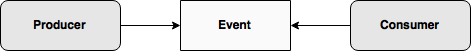
\includegraphics[scale=0.65]{chap3/images/event.png}
    % event.png: 472x52 pixel, 72dpi, 16.65x1.83 cm, bb=0 0 472 52
  \end{center}
  \caption{Event}
  \label{fig:event}
\end{figure}
 %An event is a notification that a happening of interest has occurred \cite{glossary}. Examples are a purchase order, an email confirmation of an airline reservation, a stock tick message that reports a stock trade, a message that reports a sensor reading or a smart meter alarm. 
 \subsection{Event type}
 An event type is an expression that characterizes a class of significant facts (events) and the context under which they occur. Facts of the same nature are denoted by events that have the same type. Event types are characterized by an event model. An event model gives concepts and general structures used to represent event types.

According to the complexity of the event model, the event types are represented as sequences of strings \cite{Yuhara1994}, regular expressions \cite{Bailey1994} or as expressions of an event algebra \cite{Chakravarthy1994, Gatziu1994, Collet96}. Otther models represent an event type as a collection of parameters or attributes, allowing the type itself to contains implicitly the content of the message. For example, \textit{MeterAlarm(idMeter:string, voltage:real, current:real)} is an event type that represents a smart meter reading, where the current and voltage values observed are represented by attributes \textit{voltage} and \textit{current}.

We represent an event type as a collection of attributes:\\
$EventType E:= Set <Attribute>. \\
Attribute:= <Name, Value>.
$

The definition of an event type includes the attributes presented in Table \ref{tab:evtAttributes}. The \textit{typeName} attribute refers to the name of the event type. The \textit{producerID} attribute refers to the id of the entity that produced the event occurence. The \textit{detectionTime} attribute refers to the time at which the event occurence has been detected by a source. The \textit{productionTime} attribute refers to the time at which the event has been produced (as a result of processings on others events) by an event-processing unit. The \textit{notificationTime} attribute refers to the time at which the event is notified to interested consumers. The \textit{receptionTime} attribute refers to the time at which an interested consumer receives the event. The context (\textit{context} attribute) of an event type defines all the attributes that are particular to this event type. They represent the others data manipulated by the producer, which are relevant to this event type.
\definecolor{tcB}{rgb}{1,1,1}
\definecolor{tcA}{rgb}{0,0,0}
\begin{table}[h!]
\begin{center}
\begin{tabular}{ll}
% use packages: color,colortbl
\rowcolor{tcA}
\textbf{\textcolor{tcB}{Name}} & \textbf{\textcolor{tcB}{Type}}\\
%\rowcolor{tcA}
typeName & String\\
%\rowcolor{tcA}
producerID & String\\
%\rowcolor{tcA}
detectionTime & Number\\
productionTime & Number\\
%\rowcolor{tcA}
notificationTime & Number\\
receptionTime & Number\\
%\rowcolor{tcA}
context & Set<Attribute>
\end{tabular}
\caption {Event types attributes}
\label{tab:evtAttributes}
\end{center}
\end{table}
 An event instance (or simply event) is an occurrence of an event type.
 
 \subsection{Simple event type, complex event type}
Event types can be classified as simple event types that describe elementary facts, and complex event types that describe complex situations by event combinations (see Figure \ref{fig:eventtype}). 
\begin{figure}[H]
  \begin{center}
    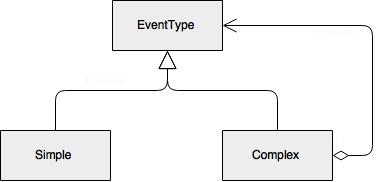
\includegraphics[scale=0.5]{chap3/images/eventType.jpg}
    % event.png: 472x52 pixel, 72dpi, 16.65x1.83 cm, bb=0 0 472 52
  \end{center}
  \caption{Classification of event types}
  \label{fig:eventtype}
\end{figure}

\subsubsection{Simple event type}
Event producers produce instances of a simple event type. Simple event instances are not generated as a result of processing others events.

\subsubsection{Complex event type}
\label{ch3:sec2.3.2}
Complex event types represent situations (relevant or critical) that can be inferred from the occurrences of others events. Complex events are produced by processing other events. Event processing operators are defined in Section \ref{ch3:sec2.3.3}.

\subsection{Event streams}
 An event stream is a continuous, append-only sequence of events. We note $Stream(s, T)$ the stream of events of type T generated by the source s. If S is a set of sources, then $\{\bigcup  stream(s,T), s \in S\}$ defines a stream of events of type T, denoted $Stream(T)$.
 
 \section{Stream based operators}
 \label{ch3:sec2.3.3}
 Complex events are produced by processing event streams. Stream based operators (or event composition operators) specify the types of operations that can be performed on event streams. In general, an event stream composition operator $op$ takes one or many input event streams of a given type, and produces an output stream of a given type (see Figure \ref{fig:op}).
 \begin{figure}[H]
  \begin{center}
    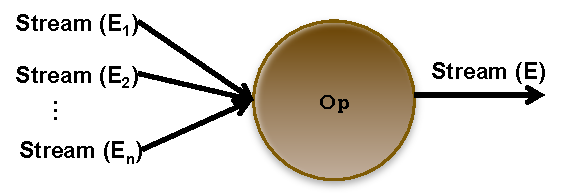
\includegraphics[scale=0.65]{chap3/images/op.pdf}
    % event.png: 472x52 pixel, 72dpi, 16.65x1.83 cm, bb=0 0 472 52
  \end{center}
  \caption{Operator synopsis}
  \label{fig:op}
\end{figure}

  \subsection{Filter}
  The \textit{filter} operator noted $filter (ES_i, P)$ takes one input stream $ES_i$ and a Predicate $P$, and produces an event $e$ in the output event stream each time an event $e_i$ in the input stream satisfies the predicate $P$, that is if $P(e_i)= true$; The context of the output event $e$ is the same as the context of the input occurrence $e_i$.
  That is, $e.context = e_i.context$.
 \subsection{Logic operators}
 Logic operators produce an event stream based on the occurrence of events in input streams.
 
 \subsubsection{Disjunction}
 The disjunction operator noted $OR(ES_1, ES_2, …, ES_n)$ produces events in the output stream at the occurrence of events in any of the input streams $ES_i, i \in \{1, 2, …,n\}$. An event $e$ is produced in the output stream if an instance $e_i$, of any input stream $ES_i$ occurs. The context of the complex event $e$ contains all occurrences $e_i$ that occur.
 
  \subsubsection{Conjunction}
  The conjunction operator noted $AND(ES_1, ES_2, …, ES_n)$ produces events in the output stream at the occurrence of events in all of the input streams $ES_i, i \in \{1, 2, …,n\}$. An event $e$ is produced in the output stream if events $e_1, e_2, …, e_n$ occur respectively in input streams $ES_1, ES_2, …, ES_n$, regardless their occurrence order. The context of the complex event $e$ contains all events $e_1, e_2, …, e_n$.
 
 \subsection{Sequence}
 The sequence operator, noted $SEQ(ES_1, ES_2, …, ES_n)$  takes two or more input event streams $ES_1, ES_2, … ES_n$ and produces a complex event $e$ in output stream each time instances $e1$ in $ES_1$, $e_2$ in $ES_2$,…, $e_n$ in $ES_n$ are received in the specified order. 
 Then, sequence denotes that $\forall i$, occurrence $e_i$ “is received before” occurrence $e_{i+1}$. 
 This implies that the reception time of event $e_1.receptionTime < e_2.receptionTime < …< e_n.receptionTime$.
 The context of the complex ec contains all events $e_1$ and $e_2$, …, $e_n$. 
 
 \subsection{Windows}
 Windows partition an event stream into finite parts $Stream_f(E)$ of the original event stream. The result is a stream of finite streams, which we note $Stream(Stream_f(E))= \{ES_{f,1}, ES_{f,2}, ES_{f,3}, ...\}$.
 The way each finite stream is constructed depends on the window specification, which can be \textit{time-based} or \textit{tuple-based}.
 \subsubsection{Time based windows}
Time based windows define windows using time intervals. 

\begin{itemize} 
\item \textbf{Fixed windows}: $win:within(t_b, t_e, ES)$. Defines a fixed time interval $[t_b, t_e]$. The output stream contains a single finite event stream $ES_{f,1}$ such that $\forall e \in ES, e \in ES_{f,1}$ iff $t_b \leq e_i.receptionTime \leq t_e $ .
\item \textbf{Landmark windows}: $win:since(t_b, ES)$. Defines a fixed lower bound time $tb$. The output stream is a sequence of finite event streams $ES_{f,i}, i \in \{1, 2, …, n\}$, such that each $ES_{f,i}$ contains events $e_i$ received since the time lower bound $t_b$. That is, $\forall i, e \in ES_{f,i}$ iff $t_b \leq e_i.receptionTime$.
\item \textbf{Sliding windows}: $win:sliding(t_w, t_s, ES)$. Defines a time duration $t_w$ and a time span $t_s$. The output stream
is a sequence of finite event streams  $ES_{f,i}, i \in \{1, 2, …, n\}$, such that each $ES_{f,i}$ contains events from stream $ES$ produced 
during last $t_w$ time units. The finite event streams in the sequence are produced each $t_s$ time unit. That is, if $ES_{f,i}$ is produced at time t, then $ES_{f,i+1}$ will be produced at time $t+t_s$. 
\end{itemize}

\subsubsection{Size bounded windows}
A size bounded window defines the number of events for each window. We distinguish between size fixed windows and sliding size fixed windows.
\begin{itemize}
 \item \textbf{Size fixed windows}: $win:batch(nb, ES)$. Specifies a fixed size \textit{nb} of each finite stream. The output stream is a sequence of finite event streams $ES_{f,i}, i \in \{1, 2, …, n\}$, such that each finite event stream $ES_{f,i}$ contains $nb$ most recent events from $ES$, and are non-overlapping. If we consider the event stream $ES = \{e_1, e_2, e_3, e_4, e_5, e_6, …\}$, $win:batch(3, ES)$ will result in finite event streams $\{ES_{f,1}, ES_{f,2},...\}$ such that $ES_{f,1} = \{ e_1, e_2, e_3\}$, $ES_{f,2} = \{ e_4, e_5, e_6\}$, and so on. 

 \item \textbf{Moving fixed size windows}: $win:mbatch (nb, m, ES)$. Defines a fixed size $nb$ of each finite stream, and a number of events $m$ after which the window moves. The output stream is a sequence of finite event streams $ES_{f,i}, i \in \{1, 2, …, n\}$, such that each $ES_{f,i}$ contains $nb$ most recent events from $ES$. $ES_{f,i+1}$ is started after $m$ events are received in $ES_{f,i}$ (moving windows). As result, an event instance may be part of many finite event streams. This is the case if $m \leq nb$. For example, if we consider windows of size nb=3 moving after each m = 2 events, that is $win:mbatch (3, 2, ES)$, the event stream $ES = \{ e_1, e_2, e_3, e_4, e_5, e_6, e_7, …\}$ will be partitioned into finite event streams $\{ES_{f,1}, ES_{f,2}, ES_{f,3} , …\}$ such that $ES_{f,1}=\{e_1, e_2, e_3\}$, $ES_{f,2} = \{ e_3, e_4, e_5\}$, $ES_{f,3} = \{e_5, e_6, e_7\}$, and so on.
\end{itemize}

\subsection{Aggregator}
Applied on a stream of finite streams $Stream(Stream_f(E))= \{ES_{f,1}, ES_{f,2}, ES_{f,3}, ...\}$, an aggregator operator $aggregate(attr, Stream(Stream_f(E_i)))$ computes for each finite stream $ES_{f,i}, i \in \{1, 2, …, n\}$, a complex event $e$ which carry (within its context) the aggregated value of the attribute \textit{attr} over events occurrences in $ES_{f,i}$. The output is a stream of such complex events. Aggregates operators include \textit{max, min, count, avg} and \textit{sum}. 
\begin{itemize}
 \item The $max$ operator compute the maximum value of the attribute over the event instances in $ES_{f,i}$.
 \item The $min$ operator compute the minimum value of the attribute over the event instances in $ES_{f,i}$.
 \item The $count$ operator compute the number of event instances in $ES_{f,i}$ with the specified attribute.
 \item The $avg$ operator compute the average value of the attribute over the event instances in $ES_{f,i}$.
 \item The $sum$ operator compute the sum of the attribute's values over the event instances in $ES_{f,i}$.
\end{itemize}

\subsection{Selection operators}
A selection operator takes as input a stream of finite streams $\{ES_{f,1}, ES_{f,2},...\}$ and produce as output an event stream ${e_1, e_2, … }$ such that for all i, each $e_i$ is a selection of a particular event from $ES_{f,i}$. The choice of that particular occurrence depends on the selection operator: %[GD93, GD94]:
\begin{itemize}
 \item \textbf{ First occurrence}: $first (Stream(Stream_f(E)))$. \\
For each finite stream $ES_{f,i}, i \in \{1, 2, …, n\}$, selects the first event occurrence. For example, if we apply the first operator to the stream of finite streams $\{\{e_1, e_2\}$, $\{ e_3, e_4, e_5, e_6\}$, $\{ e_7, e_8\},…\}$, we obtain as output the stream $\{e_1, e_3, e_7, …\}$.
   \item \textbf{Last occurrence}: $last (Stream(Stream_f(E)))$. \\
For each finite stream $ES_{f,i}, i \in \{1, 2, …, n\}$, selects the last event occurrence. For example, if we apply the last operator to the stream of finite streams $\{\{e_1, e_2\}$, $\{ e_3, e_4, e_5, e_6\}$, $\{ e_7, e_8\},…\}$, we obtain as output the stream $\{e_2, e_6, e_8, …\}$.
\end{itemize}
\subsection{Flatten}
 Flatten operator takes as input a stream of finite event streams $\{ES_{f,1}, ES_{f,2}, ES_{f,3}, ...\}$  and produce as output a stream of events constructed by concatenating events in $ES_{f,1}, ES_{f,2}, ES_{f,3}$, and so on. 
For example, if we consider the stream of finite streams $\{\{e_1\}, \{e_2, e_3\}, \{e_4, e_5, e_6\}, …\}$, the flatten operator produces the output stream $\{e_1, e, e_2, e_3,e, e_4, e_5, e_6, e, …\}$ where $e$ is a special “empty” event that indicates the end of each finite stream in the output stream.

\section{Selection policy}
\label{ch3:sec4}
% In general, stream based operators process selects one or more input event streams and produce as output one event stream.
% In some cases, an operator can receive many instances of input events can be of events 
% The production of one event in the output stream 
% In general, stream-based operators select some events in input str
% perfom event per event, as event are arriving on input event streams. This is the case for the filter operator, the For example, In some cases,  
There are situations where more than one event instance from input streams can participate in the generation of a complex event in the output stream. For example, condider the situation depicted at Figure \ref{fig:selectionpolicy} where the \textit{and} operator is performed on two event streams A and B. Suppose that two event occurrences $a_1$ and $a_2$ are received from input stream A at time $t_1$ and $t_2 > t_1$ respectively. According to the operator semantic, a complex event has to be produced in the output stream when occurrences from input streams A and B are received. So, at time $t_2$, there is nothing produced in the output. Now let's suppose that an occurrence $b_1$ is received from input stream B at time $t_3 > t_2$. Now, the \textit{and} operator should produce a composite event in the output. For that, it must be specified which occurrence between $a_1$ and $a_2$ should be considered for the construction of the complex event. It is the goal of selection policies, to specify the events to be selected in such situations. The event selection policies are classified in recent, chronologic,  continuous and cumulative.

\begin{figure}[H]
  \begin{center}
    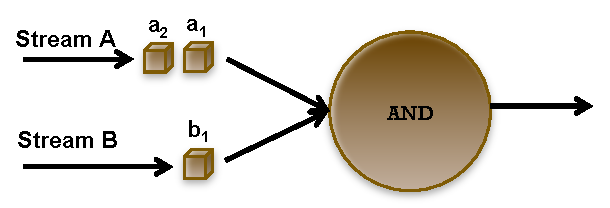
\includegraphics[scale=0.65]{chap3/images/selectionpolicy.pdf}
    % event.png: 472x52 pixel, 72dpi, 16.65x1.83 cm, bb=0 0 472 52
  \end{center}
  \caption{Example situation where a selection policy should be applied}
  \label{fig:selectionpolicy}
\end{figure}
\begin{description}
  \item[Recent]  Only the newest event occurence is selected. In the example depicted in Figure \ref{fig:selectionpolicy}, the event $a_2$ is selected between $a_1$ and $a_2$.
  \item[Chronologic]  Only the oldest event occurence is selected. In the example depicted in Figure \ref{fig:selectionpolicy}, the event $a_1$ is selected between $a_1$ and $a_2$.
  \item[Continuous] All the event occurences are selected. In the example depicted in Figure \ref{fig:selectionpolicy}, the event $a_1$ and $a_2$ are selected. As result, two complex events are produced in the output stream, with event parameters \{$a_1$, $b_1$\} and \{$a_1$, $b_2$\} respectively.
  \item[Cumulative]  All the event occurrences are accumulate in order to produce the complex event. In the example depicted in Figure \ref{fig:selectionpolicy}, the event $b_1$ is combined with both events $a_1$ and $a_2$.
\end{description}

 \section{Event composition graph}
 \label{ch3:sec5}
 As mentionned is Section \ref{ch3:sec2.3.2}, complex events are produced by processing event streams. A complex event is specified using an \textit{event composition graph}. As illustrated in Figure \ref{fig:ecg}, an event composition graph identify the event streams to be processed with the operation chain to be performed on them. More formally, an event composition graph is a direct acyclic graph (DAG) $G=<\mathcal{N}, \mathcal{S}>$, where $\mathcal{N}= \{P \cup O\}$ consists in terminal nodes $P$ and non-terminal nodes $O$, and the edge set $\mathcal{S}$. Terminal nodes $P$ represent input stream producers and non-terminal nodes $O$ represent stream based operators. The edges $\mathcal{S}$ represent event streams. Event composition graphs can be specified using either a graphical user interface, or programmaticaly. In this thesis, we only consider their internal representation as DAGs.% with less focus on how such DAG can be defined from an end user point of view.   
 \begin{figure}[H]
  \begin{center}
    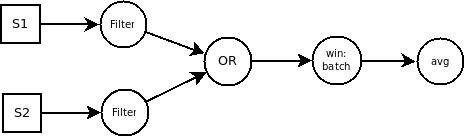
\includegraphics[scale=0.65]{chap3/images/ecg.jpg}
    % event.png: 472x52 pixel, 72dpi, 16.65x1.83 cm, bb=0 0 472 52
  \end{center}
  \caption{Event composition graph}
  \label{fig:ecg}
\end{figure}
 
 \section{Quality of service}
 \label{ch3:sec-three}
 Event streams composition in smart grids face many challenges that are due to QoS that have to be guaranteed. This section first discusses such QoS requirements and then, presents how they modeled as QoS expressions.              
\subsection{QoS dimensions}
The quality of serice dimensions that we identify as relevant for smart grids are:
\begin{itemize}
 \item \textit{Latency}. Once detected, events may have to be notified as fast as possible to consumers. Such a timing constraint is even critical in some applications. For example, in the common practice for power device protection, the circuit breaker must be opened immediately if the voltage or current on a power device exceeds the normal values. The notification latency of an event is the time elapsed between its production and its notification to interested consumers.
%The notification latency of an event is the time elapsed between its production and its notification to interested consumers. 
%The notification latency constraint imposed on an event processing unit defines an upper bound on the notification latency of events produced by that event processing unit.
%The notification latency QOS criteria associated with an event defines an upper bound on its notification latency
%In SoGrid, the notification of an event can be immediate (low latency) or delayed (high latency)

 \item \textit{Event priority}. Event priority defines a priority order between events. In some contexts, there may exist priorities between events that have to be captured by the event processing runtime. For example in a smart grid, alarm events are generally higher priority than events that report energy consumption. Events that have a higher priority have to be processed and notified earlier than less priority events.

 \item \textit{Memory occupation}. Different devices may have different available memory capacities. To adapt the event processing to the memory capacity of each device, it must be a way to specify the maximum memory occupation incurred by an event processing unit at the execution time. The memory occupation constraint gives an upperbound on the number of events that an event processing unit can maintain in its main memory at execution time.
\end{itemize}

\subsection{QoS expression}
Let's consider three domains $D_{latency}$, $D_{priority}$, $D_{memory}$, corresponding to the QoS dimensions latency, event prioity and memory occupation respectively.
Those domains are described below:
%The domains corresponding to the QoS criteria we considered are described below:
\begin{itemize}
 \item $D_{latency} \subseteq R+$, as the latency corresponds to a time delay (an expected value for measuring time belongs to the set of positive real numbers). The domain inherits the properties of R+ (e.g. the operators of comparison). Best is shortest for latencies, the latency is bounded with the comparison operator ``less than'' (<) and ``less or equal to'' ($\leq$). 
 \item $D_{priority} \subseteq N*$. An event type is associated to a priority level. The lower is the priority level, the higher is the priority associated to the event. The priority level varies according to the event type. The domain inherits the properties of $N$ (e.g. the operators of comparison). 
 The priority is heavily restricted bounded, thus ``equal to'' (=) is the only accepted comparison operator.
 \item $D_{memory}  \subseteq N$, as the memory corresponds to a quantity. The domain inherits the properties of $N$. The memory occupation is associated to an upper-bound that indicates the maximum memory available on a processing device. This is denoted by the comparison operator ``less or equal to'' ($\leq$).  
\end{itemize}
Let us assume $D$ the set of the QoS domains that we considered, that is $D = D_{latency} \bigcup D_{priority} \bigcup D_{memory}$.
Given a domain $D_Q$, we assume a function \textit{name($D_Q$)} that returns its  name, a function \textit{operator($D_Q$)} that returns the set of related operators, and a function \textit{value($D_Q$)} that returns the set of included values.
For instance, let us consider the domain $D_{priority}$, thus: 
\begin{itemize}
 \item \textit{name($D_{piority}$)} = event priority,
 \item \textit{operator($D_{priority}$)} = { equal to (=) },
 \item \textit{value($D_{latency}$)} = $N*$, this is the set of all positive integer numbers.
\end{itemize}
Let also consider that $\mathcal{L}$ is the set of available processing devices.
\subsubsection{Atomic QoS expression} 
An atomic QoS expression is of the form $(d, \theta, v)$ or , $(d, \theta, v, l)$ where 
\begin{itemize}
 \item d denotes a domain $D_Q , D_Q \in D$,
 \item $\theta \in$ \textit{operator($D_Q$)},
 \item $v \in$ \textit{value($D_Q$)},
 \item $l \in \mathcal{L}$ is a processing device.
\end{itemize}
For instance, the atomic QoS (latency, $\leq$, 2000) specifies that the latency for notifying an event must be less or equal to 2000 ms, assuming that the time unit is the millisecond. In the same way, the atomic QoS (memory, $\leq$, 1000, device1) specifies that the memory occupation on the device ``device1'' must be less or equal to 1000 Mo, assuming that the unit for the memory is the megabyte.  

\subsubsection{Complex QoS expression} 
A complex QoS expression specifies multiple QoS criteria. It is defined inductively as follows.
\begin{enumerate}
 \item An atomic QoS is a complex QoS expression.
 \item If $QC_1$ and $QC_2$ are complex QoS expressions then $QC_1 \wedge QC_2$ is a complex QoS expression.
\end{enumerate}
 The QoS expression (latency, $\leq$, 2000) $\wedge$ (event priority, =, 1) specifies that the latency must be less than or equal to 2000 ms, and in addition, the highest priority level (i.e. priority = 1) is required.
%Dmemocc domain represent the memory occupation criterion;  Dmemocc ⊆ N ≤ m. Where  m corresponds to the maximum memory capacity of the current device. The domain inherits the properties of N. The event processing memory occupation has an upper-bound of the the number of events that an event processing unit can maintain, it is denoted by the comparison operator ‘less than or equal to’ (≤).

 \section{Conclusion}
In this chapter, we presented a model for event streams composition. We focused on the definition of concepts that are manipulated by an event stream composition system. First, we presented the concepts of event, simple and complex event types, and event streams. Then, we presented operators applicable to event streams in order to produce complex events, with their associate selection policies. After that, we presented how stream based operators can be combined together to define the event composition logic associate to a complex event. And finally, we presented some QoS dimensions applicable to an event composition, and how they can be specified using QoS expressions. 

In the next chapter, we will go one step forward, by presenting how the presented model can be leveraged to define an approach for distributed event streams composition that deals with QoS.